%% msc_thesis.tex -- document template for graduate theses at UofT
%%
%% Copyright (c) 1998-2013 Francois Pitt <fpitt@cs.utoronto.ca>
%% last updated at 16:20 (EDT) on Wed 25 Sep 2013
%%
%% This work may be distributed and/or modified under the conditions of
%% the LaTeX Project Public License, either version 1.3c of this license
%% or (at your option) any later version.
%% The latest version of this license is in
%%     http://www.latex-project.org/lppl.txt
%% and version 1.3c or later is part of all distributions of LaTeX
%% version 2005/12/01 or later.
%%
%% This work has the LPPL maintenance status "maintained".
%%
%% The Current Maintainer of this work is
%% Francois Pitt <fpitt@cs.utoronto.ca>.
%%
%% This work consists of the files listed in the accompanying README.

%% SUMMARY OF FEATURES:
%%
%% All environments, commands, and options provided by the `ut-thesis'
%% class will be described below, at the point where they should appear
%% in the document.  See the file `ut-thesis.cls' for more details.
%%
%% To explicitly set the pagestyle of any blank page inserted with
%% \cleardoublepage, use one of \clearemptydoublepage,
%% \clearplaindoublepage, \clearthesisdoublepage, or
%% \clearstandarddoublepage (to use the style currently in effect).
%%
%% For single-spaced quotes or quotations, use the `longquote' and
%% `longquotation' environments.


%%%%%%%%%%%%         PREAMBLE         %%%%%%%%%%%%

%%  - Default settings format a final copy (single-sided, normal
%%    margins, one-and-a-half-spaced with single-spaced notes).
%%  - For a rough copy (double-sided, normal margins, double-spaced,
%%    with the word "DRAFT" printed at each corner of every page), use
%%    the `draft' option.
%%  - The default global line spacing can be changed with one of the
%%    options `singlespaced', `onehalfspaced', or `doublespaced'.
%%  - Footnotes and marginal notes are all single-spaced by default, but
%%    can be made to have the same spacing as the rest of the document
%%    by using the option `standardspacednotes'.
%%  - The size of the margins can be changed with one of the options:
%%     . `narrowmargins' (1 1/4" left, 3/4" others),
%%     . `normalmargins' (1 1/4" left, 1" others),
%%     . `widemargins' (1 1/4" all),
%%     . `extrawidemargins' (1 1/2" all).
%%  - The pagestyle of "cleared" pages (empty pages inserted in
%%    two-sided documents to put the next page on the right-hand side)
%%    can be set with one of the options `cleardoublepagestyleempty',
%%    `cleardoublepagestyleplain', or `cleardoublepagestylestandard'.
%%  - Any other standard option for the `report' document class can be
%%    used to override the default or draft settings (such as `10pt',
%%    `11pt', `12pt'), and standard LaTeX packages can be used to
%%    further customize the layout and/or formatting of the document.

%% *** Add any desired options. ***
\documentclass{ut-thesis}

%% *** Add \usepackage declarations here. ***
%% The standard packages `geometry' and `setspace' are already loaded by
%% `ut-thesis' -- see their documentation for details of the features
%% they provide.  In particular, you may use the \geometry command here
%% to adjust the margins if none of the ut-thesis options are suitable
%% (see the `geometry' package for details).  You may also use the
%% \setstretch command to set the line spacing to a value other than
%% single, one-and-a-half, or double spaced (see the `setspace' package
%% for details).


%%%%%%%%%%%%%%%%%%%%%%%%%%%%%%%%%%%%%%%%%%%%%%%%%%%%%%%%%%%%%%%%%%%%%%%%
%%                                                                    %%
%%                   ***   I M P O R T A N T   ***                    %%
%%                                                                    %%
%%  Fill in the following fields with the required information:       %%
%%   - \degree{...}       name of the degree obtained                 %%
%%   - \department{...}   name of the graduate department             %%
%%   - \gradyear{...}     year of graduation                          %%
%%   - \author{...}       name of the author                          %%
%%   - \title{...}        title of the thesis                         %%
%%%%%%%%%%%%%%%%%%%%%%%%%%%%%%%%%%%%%%%%%%%%%%%%%%%%%%%%%%%%%%%%%%%%%%%%

%% *** Change this example to appropriate values. ***
\degree{Master of Science}
\department{Computer Science}
\gradyear{2016}
\author{Alexey Strokach}
\title{Predicting the Effect of Mutations on a Genome-Wide Scale}

%% *** NOTE ***
%% Put here all other formatting commands that belong in the preamble.
%% In particular, you should put all of your \newcommand's,
%% \newenvironment's, \newtheorem's, etc. (in other words, all the
%% global definitions that you will need throughout your thesis) in a
%% separate file and use "\input{filename}" to input it here.


%% *** Adjust the following settings as desired. ***

%% List only down to subsections in the table of contents;
%% 0=chapter, 1=section, 2=subsection, 3=subsubsection, etc.
\setcounter{tocdepth}{2}

%% Make each page fill up the entire page.
\flushbottom



%%%%%%%%%%%%      AS CUSTOM CONFIGURATIONS      %%%%%%%%%%%%

% Source:
\usepackage{float}
\usepackage{subcaption}
\usepackage{graphicx}
\graphicspath{ {images/} }
\usepackage{booktabs}
\usepackage{hyperref}

\pdfsuppresswarningpagegroup=1


% Source: http://tex.stackexchange.com/a/110854/66387
\newcommand{\mychapter}[2]{
	\setcounter{chapter}{#1}
	\setcounter{section}{0}
	\chapter*{#2}
	\addcontentsline{toc}{chapter}{#1 #2}
}       % before-code




%%%%%%%%%%%%      CONFIGURE BIBLIOGRAPHY      %%%%%%%%%%%%

% % % % % % % % % % % % % % % % % % % % % % % % % % % % % % % % % % % % % % % % %

\usepackage[
    backend=biber,
    style=numeric,
    natbib=true,
    maxnames=2,
    sorting=nyt,
    sortcites=false,
    block=space,
    date=long,
    url=false,
    doi=true,
    eprint=false,
    isbn=false,
    uniquename=false,
    uniquelist=false,
    terseinits=true,
    giveninits=false
]{biblatex}
% \addbibresource{http://localhost:23119/better-bibtex/collection?/0/MSc thesis.biblatex}
\addbibresource{msc_thesis.bib}

\ExecuteBibliographyOptions{%
  citetracker=true,% Citation tracker enabled in order not to repeat citations, and have two lists.
  sorting=none,% Don't sort, just print in the order of citation
  alldates=long,% Long dates, so we can tweak them at will afterwards
  dateabbrev=false,% Remove abbreviations in dates, for same reason as ``alldates=long''
 % articletitle=true,% To have article titles in full bibliography
  maxcitenames=999% Number of names before replacing with et al. Here, everyone.
}

% % % % % % % % % % % % % % % % % % % % % % % % % % % % % % % % % % % % % % % % %

%%%%%%%%%%%%      MAIN  DOCUMENT      %%%%%%%%%%%%

\begin{document}

%% This sets the page style and numbering for preliminary sections.
\begin{preliminary}

%% This generates the title page from the information given above.
\maketitle

%% There should be NOTHING between the title page and abstract.
%% However, if your document is two-sided and you want the abstract
%% _not_ to appear on the back of the title page, then uncomment the
%% following line.
%\cleardoublepage

%% This generates the abstract page, with the line spacing adjusted
%% according to SGS guidelines.
\begin{abstract}
%% *** Put your Abstract here. ***
%% (At most 150 words for M.Sc. or 350 words for Ph.D.)
\end{abstract}

%% Anything placed between the abstract and table of contents will
%% appear on a separate page since the abstract ends with \newpage and
%% the table of contents starts with \clearpage.  Use \cleardoublepage
%% for anything that you want to appear on a right-hand page.

%% This generates a "dedication" section, if needed -- just a paragraph
%% formatted flush right (uncomment to have it appear in the document).
%\begin{dedication}
%% *** Put your Dedication here. ***
%\end{dedication}

%% The `dedication' and `acknowledgements' sections do not create new
%% pages so if you want the two sections to appear on separate pages,
%% uncomment the following line.
%\newpage  % separate pages for dedication and acknowledgements

%% Alternatively, if you leave both on the same page, it is probably a
%% good idea to add a bit of extra vertical space in between the two --
%% for example, as follows (adjust as desired).
%\vspace{.5in}  % vertical space between dedication and acknowledgements

%% This generates an "acknowledgements" section, if needed
%% (uncomment to have it appear in the document).
%\begin{acknowledgements}
%% *** Put your Acknowledgements here. ***
%\end{acknowledgements}

%% This generates the Table of Contents (on a separate page).
\tableofcontents

%% This generates the List of Tables (on a separate page), if needed
%% (uncomment to have it appear in the document).
\listoftables

%% This generates the List of Figures (on a separate page), if needed
%% (uncomment to have it appear in the document).
\listoffigures

%% You can add commands here to generate any other material that belongs
%% in the head matter (for example, List of Plates, Index of Symbols, or
%% List of Appendices).

%% End of the preliminary sections: reset page style and numbering.
\end{preliminary}


%%%%%%%%%%%%%%%%%%%%%%%%%%%%%%%%%%%%%%%%%%%%%%%%%%%%%%%%%%%%%%%%%%%%%%%%
%%  Put your Chapters here; the easiest way to do this is to keep     %%
%%  each chapter in a separate file and `\include' all the files.     %%
%%  Each chapter file should start with "\chapter{ChapterName}".      %%
%%  Note that using `\include' instead of `\input' will make each     %%
%%  chapter start on a new page, and allow you to format only parts   %%
%%  of your thesis at a time by using `\includeonly'.                 %%
%%%%%%%%%%%%%%%%%%%%%%%%%%%%%%%%%%%%%%%%%%%%%%%%%%%%%%%%%%%%%%%%%%%%%%%%

%% *** Include chapter files here. ***
% !TEX root = msc_thesis.tex

\chapter{Introduction}

\section{Background}

Recent advances in DNA sequence technology have drastically lowered the cost and improved the accuracy of genome sequencing \cite{wetterstrand_dna_2016}. This has made exome and whole-genome sequencing a viable and cost-effective tool in both the laboratory and in the clinic to assist with the diagnosis and direct treatment of pediatric conditions \cite{chrystoja_whole_2014} and cancers \cite{nik-zainal_landscape_2016}, and has led to an enormous growth in the amount of genomic data that is being generated. However, interpreting such genomic data to produce meaningful and actionable results remains a challenge.

\textit{In vitro} and \textit{in vivo} experiments remain the gold standard in elucidating the effect of mutations. However, evaluating experimentally the effect of all discovered mutants is not feasible. Computational techniques have been developed to predict the effect of different mutations and to prioritize them for experimental validation. Those techniques generally use conservation score describing the likelihood that a particular amino acid being found in the particular position in orthologous proteins.

The most widely-used program for predicting the deleteriousness of a mutation is Sorting Intolerant from Tolerant (SIFT) \cite{ng_sift:_2003}. SIFT runs PSI-Blast to create a multiple sequence alignment for the query protein, and computes a conservation score by looking at the likelihood of the wildtype and mutant amino acids occurring at a given position in the alignment. While SIFT is a well-established tool in the field, it is difficult to compile and install on a local machine. Furthermore, multiple sequence alignments constructed by SIFT can be several megabytes in size, and caching this data for an entire proteome would require a non-trivial amount of storage space.

Another popular sequence-based algorithm is Provean \cite{choi_predicting_2012}. Provean also calculates uses PSI-Blast to calculate a multiple sequence alignment. However, it then runs CD-HIT to select under 100 representative sequences capturing the diversity of the alignment, and then performs pairwise alignments with this ``supporting set'' to predict the final score. Provean is reported to achieve similar performance to SIFT. However, unlike SIFT, it is freely available under the GPLv3 license, it compiles easily and runs on modern Linux distributions. Furthermore, Provean is distributed under a  license, and uses \textit{supporting sets} of at most 45 sequences which can be precalculated and stored. If a supporting set is available, calculating the Provean score takes several seconds per mutation.

The performance of Provean is comparable to the leading mutation scoring programs, such as SITF, PolyPhen-2, Mutation Assessor, and CONDEL \cite{choi_predicting_2012}. Furthermore, Provean is distributed under a GPLv3 license, and uses \textit{supporting sets} of at most 45 sequences which can precalculated and stored. If a supporting set is available, calculating the Provean score takes several seconds per mutation.

Another widely-used mutaiton scoring tool is PolyPhen-2. It is one of the packages predicted for

Many other tools have been developed that offer various advantages over SIFT / Provean. PolyPhen-2 \cite{adzhubei_predicting_2001} uses support vector machines to combine a conservation score with different sequential and structural features of the wildtype and mutant residue. However, since PolyPhen-2 is trained on a dataset of human deleterious mutations, it is difficult to use in downstream applications, as one would have to make sure to exclude the PolyPhen-2 training set throughout the training and validation process. FATHMM \cite{shihab_ranking_2014} constructs a hidden Markov model based on the alignment, and is reported to achieve marginally higher accuracy than SIFT / Provean. Other techniques offering various advantages over SIFT / Provean include MutPred \cite{li_automated_2009}, MutationAssesor \cite{network_integrated_2011}, CADD \cite{kircher_general_2014}, CONDEL \cite{choi_predicting_2012}, and others.

Despite the proliferation of tools predicting the deleteriousness of different SNPs, our ability to act on those predictions remains limited. Existing computational methods are limited in their accuracy and the type of information that they can provide. Most existing tools use a conservation score. While millions of single nucleotide polymorphisms (SNPs) have been implicated in thousands of diseases, approaches for predicting the phenotypic effect of newly-discovered mutations are still in their infancy. One of the reasons is that while sequence-based tools achieve reasonably good performance at predicting whether or not a given mutation is going to be deleterious, they fall short in predicting \textit{why} that mutation is deleterious. This lack of actionable predictions limits the usability of the vast DNA sequencing data that has been generated. However, the etiology by which the mutations cause or contribute to a disease are often unknown.



\section{Structural approaches to predicting the effect of mutations}

Statistical potentials

Physics-based methods
the electrostatic, van der Waals, solvent accessible surface area, and entropy terms

Concoord/Poisson-Boltzmann surface area (CC/PBSA server)

The central dogma of biology is that DNA is transcribed into RNA which is translated into Protein.

One reason for out lack of ability in interpreting is the focus on the sequence-level features, while in the majority of missense mutations, it is the alteration in the function of the transcribed protein which is responsible for the detrimental effect of mutations.

The field of protein science has generally been concerned with the broad questions of protein folding, protein design. Algorithms have been developed to predict the effect of mutations on protein folding and protein-protein affinity, but those tools are generally meant to be used on a case-by-case basis and have not been designed to be applied on a genome-wide scale to predict the effect of missense mutations from whole-genome sequencing studies.

While the growth in protein crystal structures has not seen the rapid rise that was observed in DNA sequencing, the number of resolved protein structures has also been increasing, with the Protein Data Bank (PDB) containing close to 125,000 structures as of 2016.

A related are of research is predicting the energetic effect of mutations.

The most accurate class of computational techniques are alchemical free energy calculations, which involve modelling the structural transition from the wildtype to the mutant protein and using the Bennett acceptance ratio (BAR) or thermodynamic integration (TI) to calculate the energetics of the transition \cite{monticelli_introduction_2013}. However, alchemical free energy calculations are computationally expansive, and are generally used only in cases where the experimental characterization of mutants is particularly difficult, as in the case of D-amino acid peptide design \cite{welch_potent_2007}.

Many algorithms have been developed which attempt to predict the effect of mutations on protein stability and / or on protein-protein interaction affinity. Those techniques generally use a rigid backbone representation of protein and use statistical potentials. For a review see XXX.

Mixed strategies which utilize both sequence- and structure-based approaches. Such algorithms include PoPMuSiC,

Structure-based tools which predict the effect of mutations on protein structure and / or function using features describing the three-dimensional structure of the protein. mCSM \cite{pires_mcsm:_2014} (graph-based signatures), MAESTRO \cite{laimer_maestro_2015} (multi-agent machine learning), CC/PBSA (Concoord/Poisson-Boltzmann surface area) \cite{benedix_predicting_2009},

Some algorithms rely on the conservation of the residue in multiple sequence alignments.

Predicting protein thermal stability changes upon point mutations using statistical potentials: Introducing HoTMuSiC

  - MAESTRO implements a multi-agent machine learning system.

  - Structure based tools AUTO-MUTE [7], CUPSAT [8], Dmutant [9], FoldX [10], Eris [11], PoPMuSiC [12], SDM [13] or mCSM [14] usually perform better than the sequence based counterparts. Recently, SDM and mCSM have been integrated into a new method called DUET [15].

INPS: predicting the impact of non-synonymous variations on protein stability from sequence

  - \url{http://bioinformatics.oxfordjournals.org/content/31/17/2816.long}

  - Here, we describe INPS, a novel approach for annotating the effect of non-synonymous mutations on the protein stability from its sequence.

  - \cite{fariselli_inps:_2015}

FoldX

PoPMuSiC

RosettaCM

mCSM: predicting the effects of mutations in proteins using graph-based signatures.

  - \url{http://www.ncbi.nlm.nih.gov/pubmed/24281696}

  - ``To understand the roles of mutations in disease, we have evaluated their impacts not only on protein stability but also on protein-protein and protein-nucleic acid interactions''.

  - \cite{pires_mcsm:_2014}


Predicting Binding Free Energy Change Caused by Point Mutations with Knowledge-Modified MM/PBSA Method

  - \url{http://journals.plos.org/ploscompbiol/article?id=10.1371%2Fjournal.pcbi.1004276}

  - ``The core of the SAAMBE method is a modified molecular mechanics Poisson-Boltzmann Surface Area (MM/PBSA) method with residue specific dielectric constant''.

  - \cite{petukh_predicting_2015}



% Benchmarks

Rosetta benchmark \cite{o_conchuir_web_2015}

Benchmark showing Rosetta doing poorly: \cite{potapov_assessing_2009}

I-Mutant2, DMutant, CUPSAT, FoldX \cite{khan_performance_2010}



\section{Goals and objectives}

\begin{itemize}
    \item Evaluate how well we can predict the deleteriousness of a mutation by measuring the effect of protein folding on protein stability.
    \item Assessing the impact of missense mutations.
    \item Protein engineering. For example generating biological therapeutics that are more thermostable and have a higher affinity for their target.
    \item Basic science: characterizing the forces that are most important in protein folding and binding, and the effect of mutations on those forces.
    \item In this work we examine how much sequence-based features can aid in the prediction of traditionally structural realms such as the prediction of $\Delta \Delta G$ scores of mutations, and how much structure-based features can aid with the prediction of mutation pathogenicity--a traditionally sequence based
\end{itemize}







\section{Acknowledgements}

This is a continuation of the work performed by Niklas Berliner \textit{et al.} \cite{berliner_combining_2014}. In \ref{chap:implementation} we discuss how we expand ELASPIC to work on the genome-wide scale. In \ref{chap:results} we discuss how we retrained ELASPIC while leveraging the information we extracted from genome-wide analysis.

% !TEX root = msc_thesis.tex

\mychapter{2}{Implementation}

\section{Training sets}

\subsection{Core}

Sanhi et al. databaset (taipale)

\subsection{Interface}


\subsection{Standalone pipeline}

\ref{fig:elaspic_pipeline} right

\section{ELASPIC pipeline}

An overview of the ELASPIC pipeline is presented in Figure \ref{fig:elaspic_pipeline}. ELASPIC includes a library Python scripts for construction sequence alignments, constructing Provean supporting sets and computing the Provean score, constructing homology models, running FoldX, and predicting the $\Delta \Delta G$ of the mutation. It also includes a ``Standalone Pipeline'' and a ``Database Pipeline'', which include command line options for mutating a protein structure.


\subsection{Standalone pipeline}

The standalone pipeline works without downloading and installing a local copy of the ELASPIC and PDB databases, but requires a PDB structure or template to be provided for every protein. Pipeline output is saves as JSON files inside the working directory, rather than being uploaded to the database as in the case of the database pipeline. The general overview of the local pipleine is presented in the figure to the right.

The local pipeline still requires a local copy of the Blast nr database.

\subsection{Database pipeline}

The database pipeline allows mutations to be performed on a proteome-wide scale, without having to specify a structural template for each protein. This pipeline requires a local copy of ELASPIC domain definitions and templates, as well as a local copy of the BLAST and PDB databases.

The general overview of the database pipleine is presented in \ref{fig:elaspic_pipeline} left. A user runs the ELASPIC pipeline specifying the Uniprot ID of the protein being mutated, and one or more mutations affecting that protein. At each decision node, the pipeline queries the database to check whether or not the required information has been previously calculated. If the required data has not been calculated, the pipeline calculates it on the fly and stores the results in the database for later retrieval. The pipeline proceeds until homology models of all domains in the protein, and all domain-domain interactions involving the protein, have been calculated, and the $\Delta \Delta G$ has been predicted for every specified mutation.

\begin{figure}[ht]
	\centering
	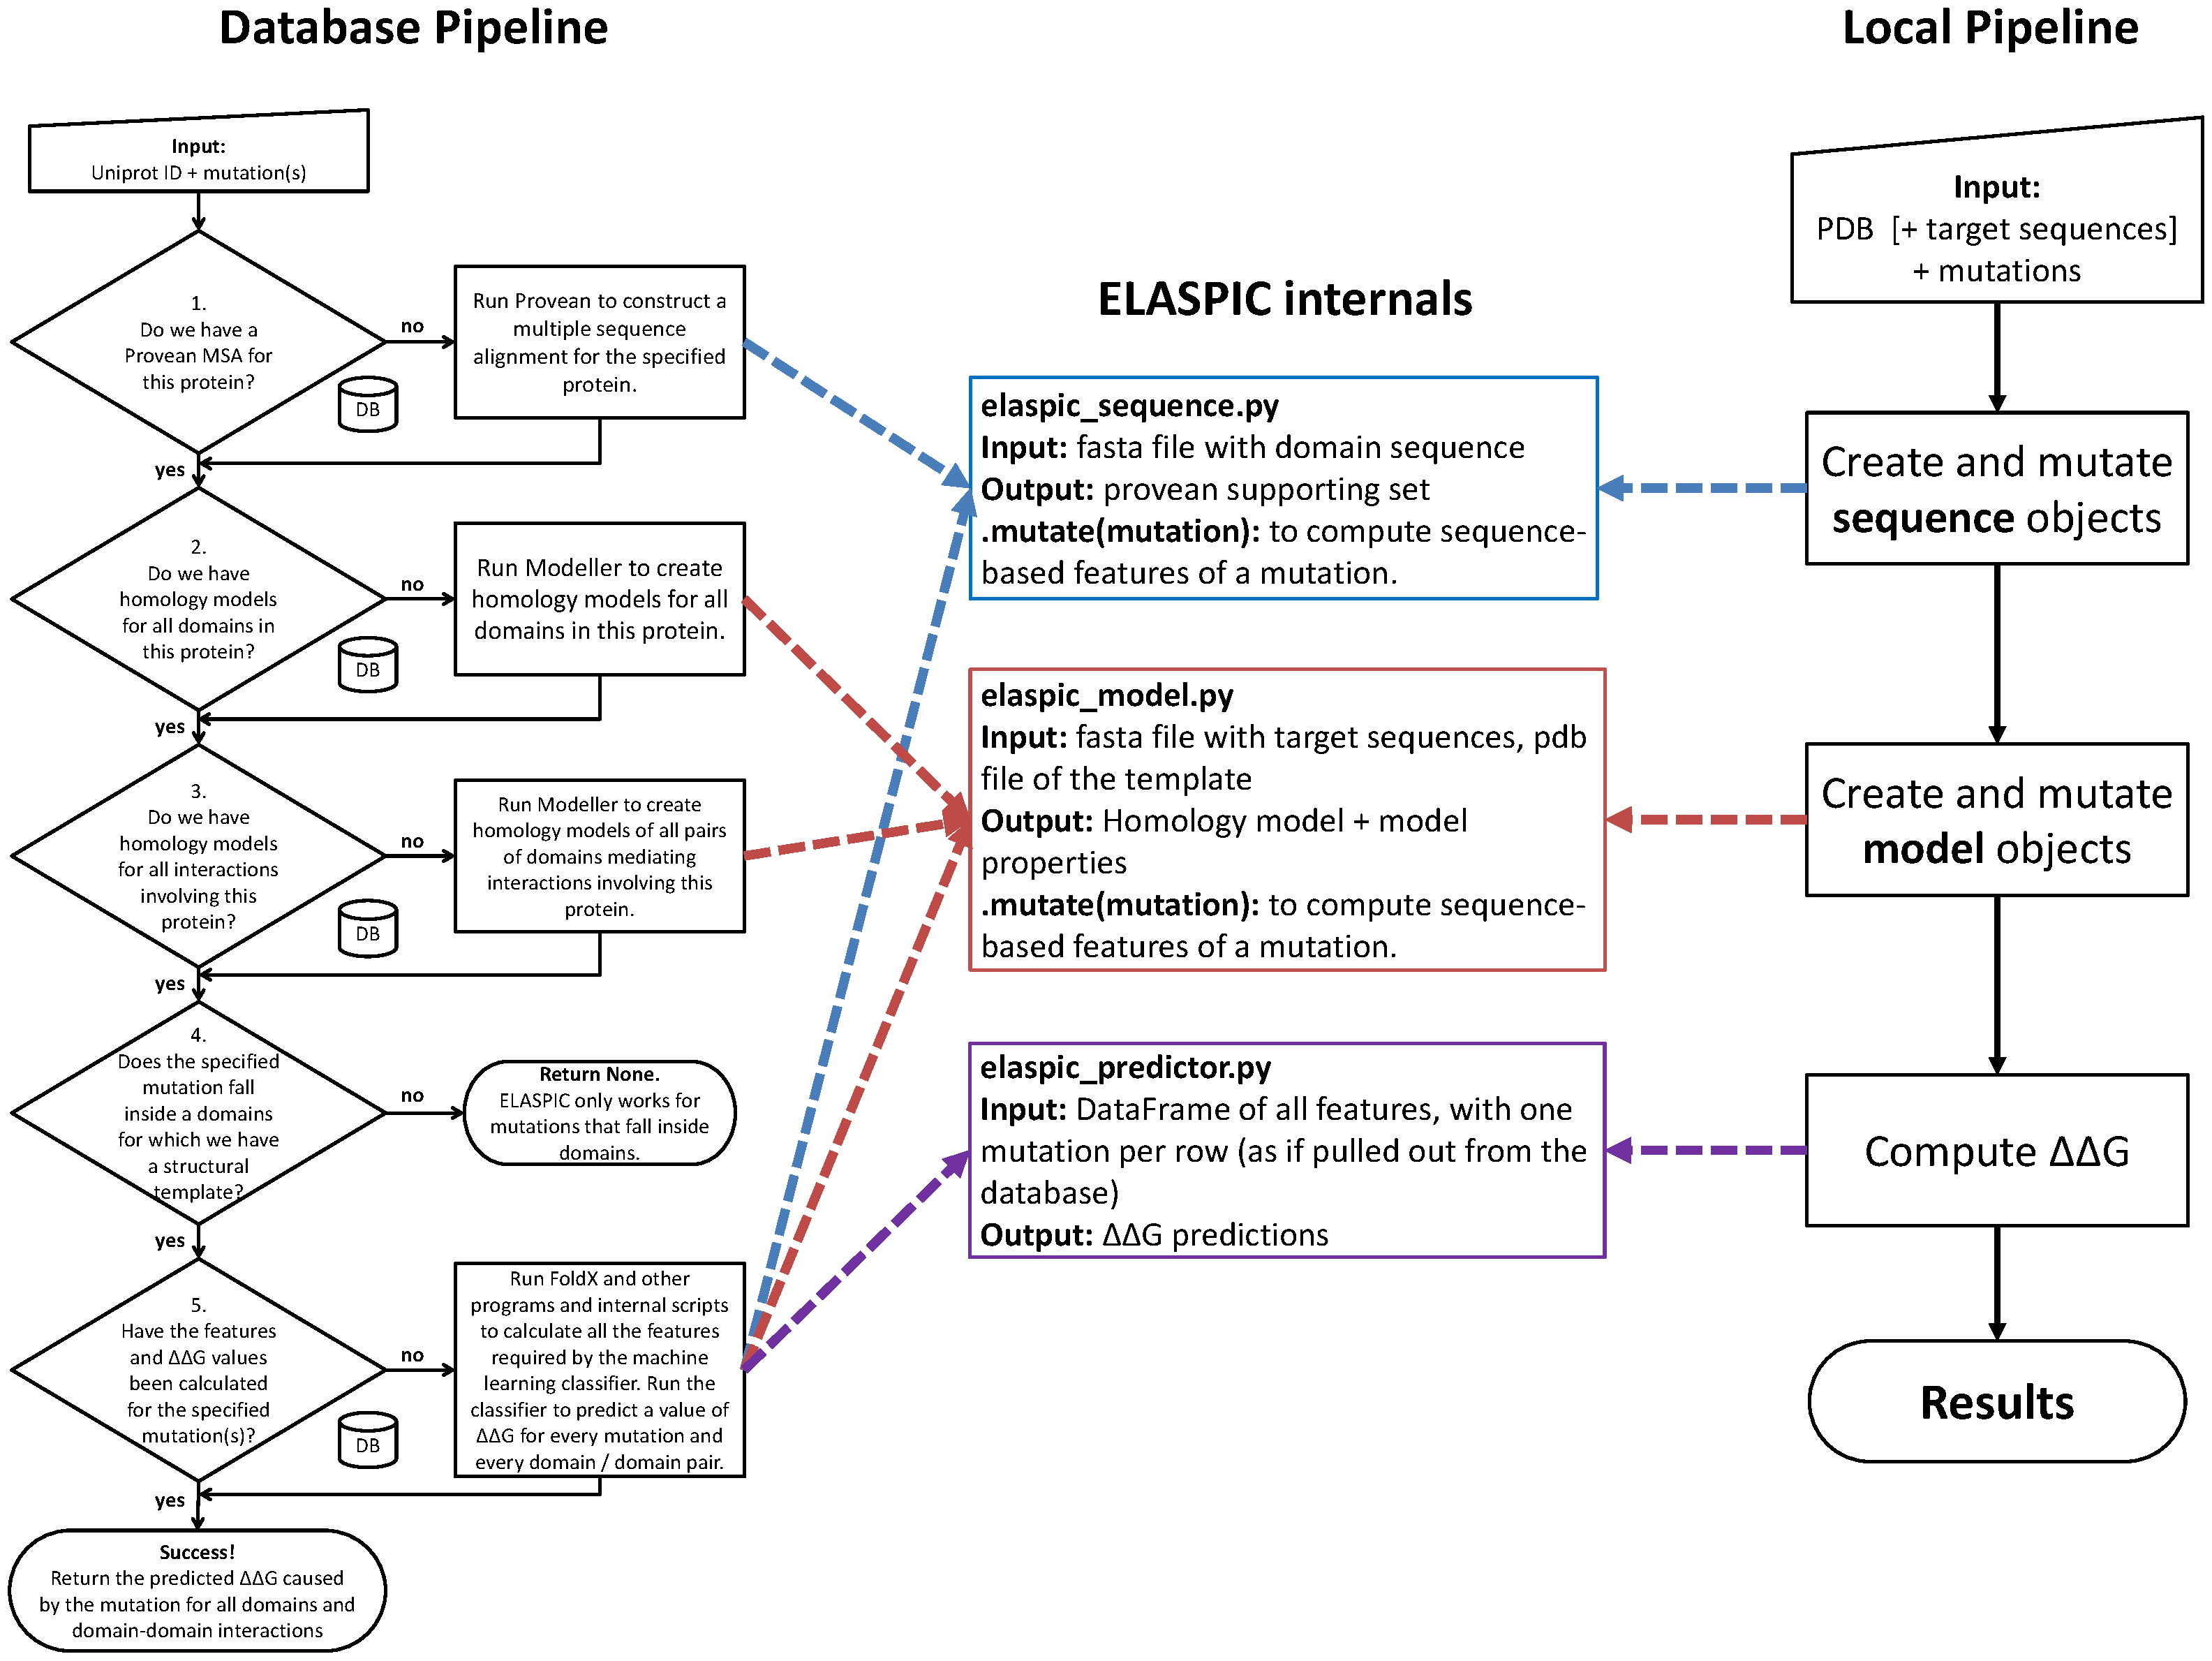
\includegraphics[width=1.0\textwidth]{static/elaspic/elaspic_flowchart.pdf}
	\caption[Overview of the ELASPIC pipeline]{Overview of the ELASPIC pipeline. A user runs the ELASPIC pipeline specifying the UniProt id of the protein being mutated, and one or more mutations affecting that protein. At each decision node, the pipeline queries the database to check whether or not the required information has been calculated previously. If the required data has not been calculated, the pipeline calculates it on the fly and stores the results in the database for later retrieval. The pipeline proceeds until homology models of all domains in the protein, and all domain-domain interactions involving the protein, have been calculated, and the $\Delta \Delta G$ has been predicted for every specified mutation.}
	\label{fig:elaspic_pipeline}
\end{figure}


\begin{figure}[ht]
	\centering
	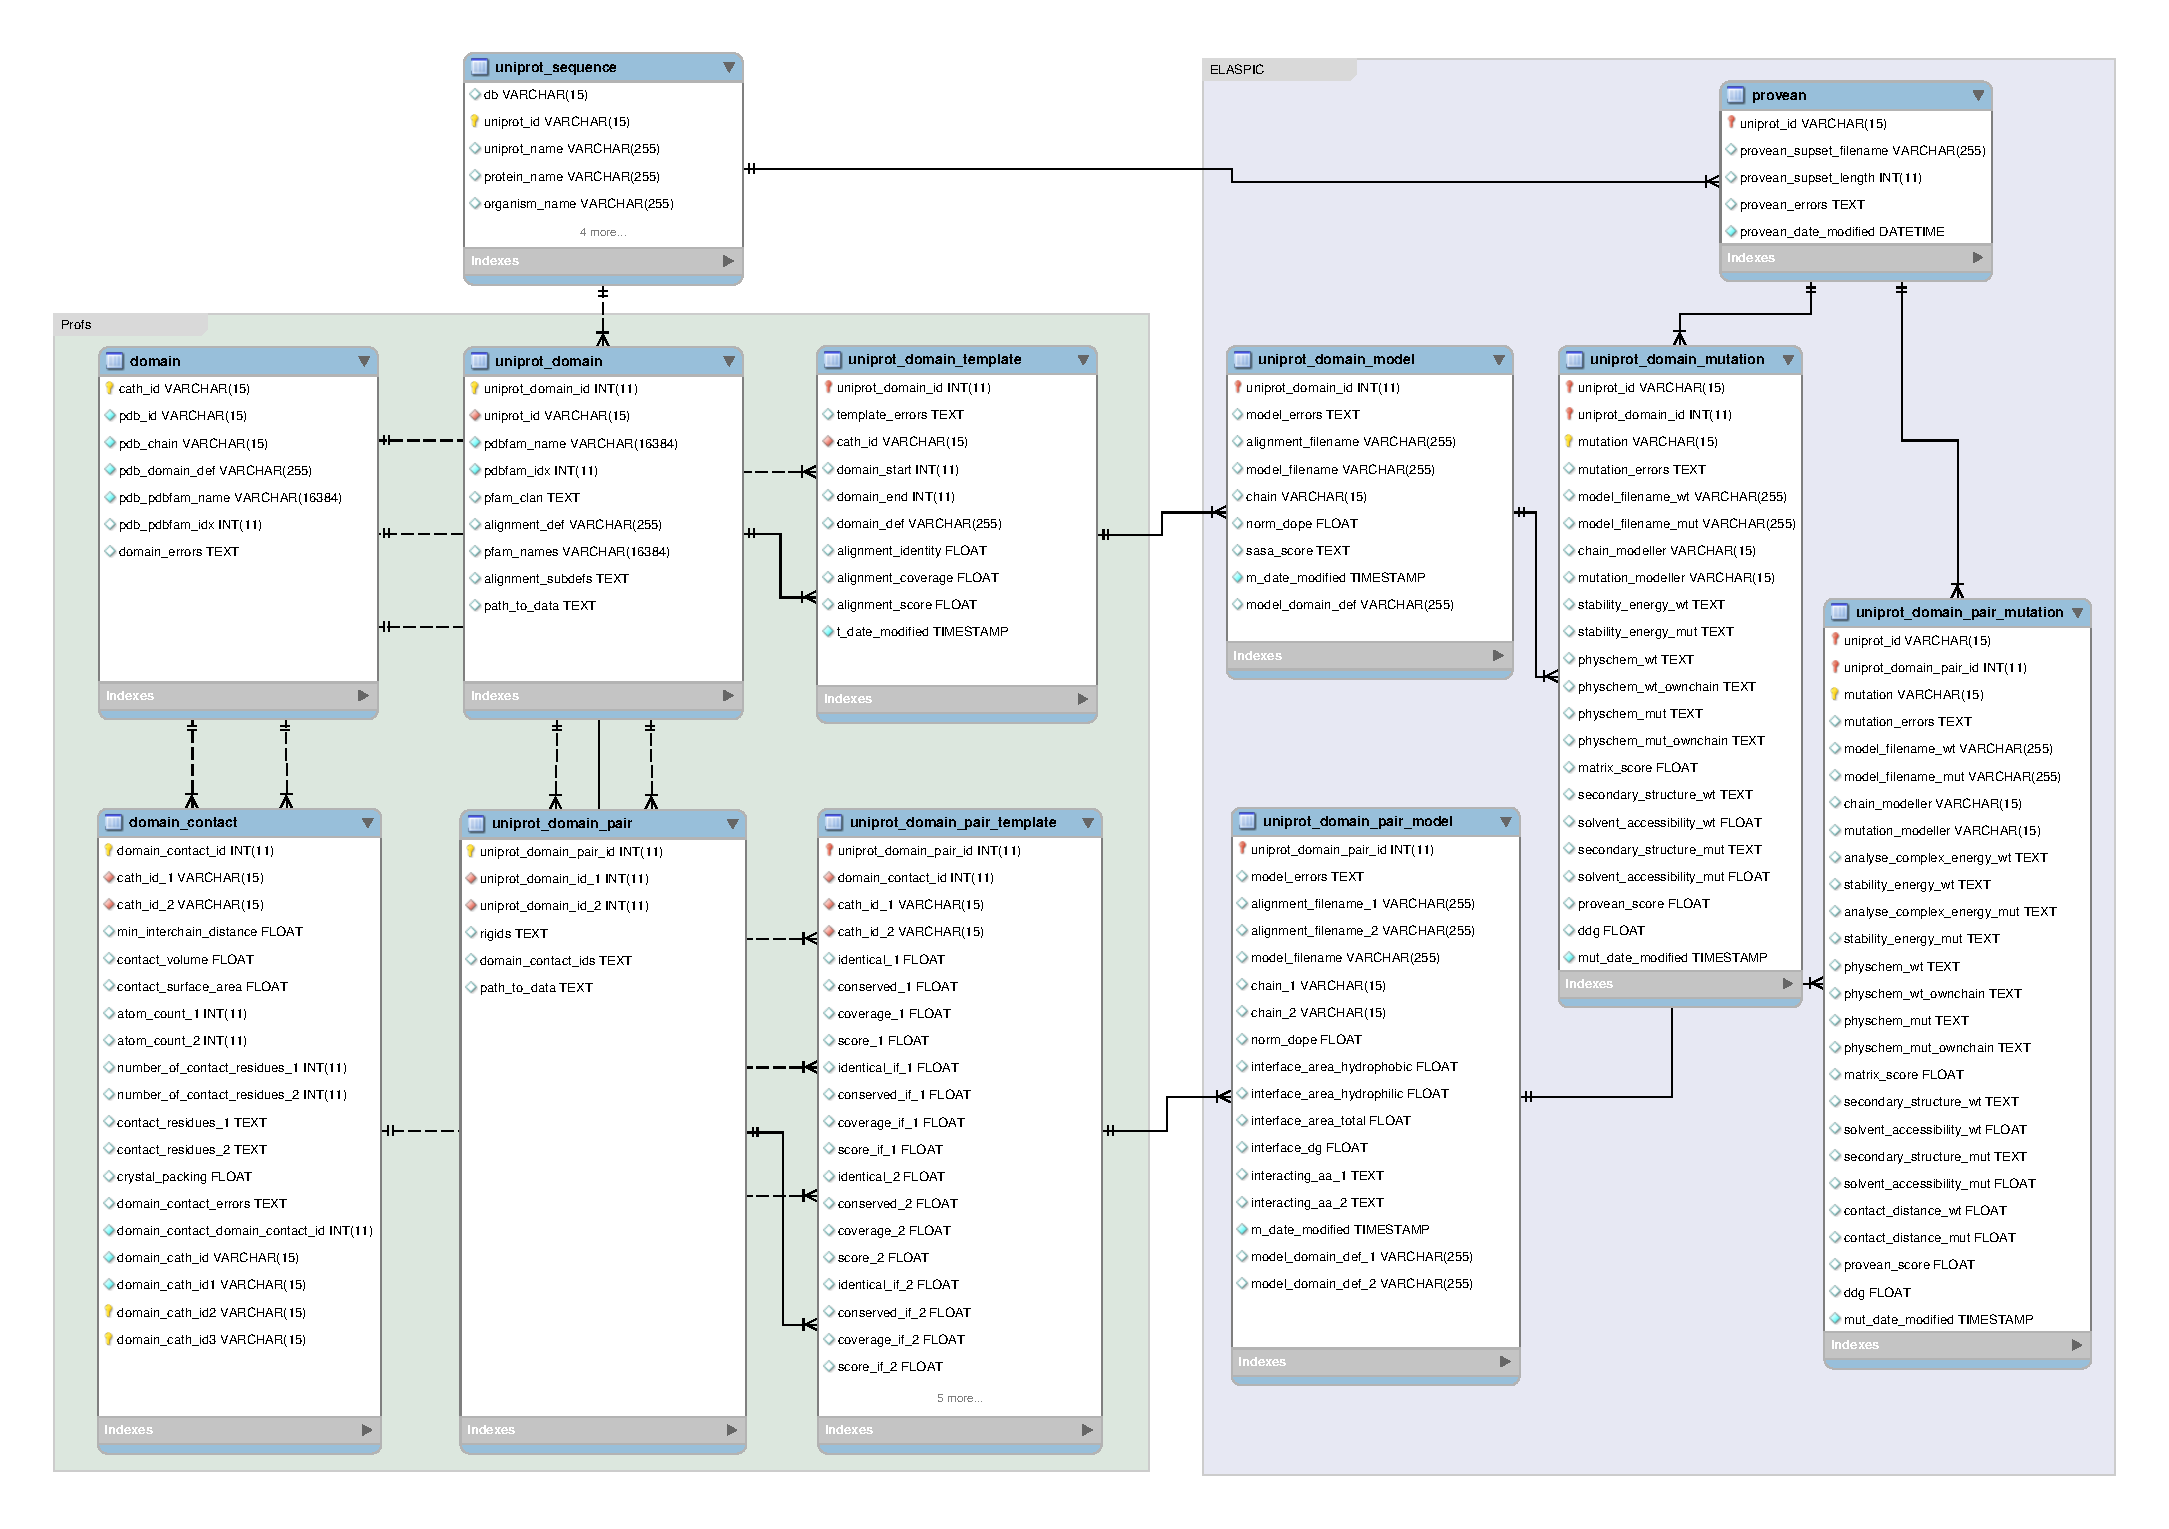
\includegraphics[width=1.0\textwidth]{static/elaspic/elaspic_schema.pdf}
	\caption{Database schema used by the ELASPIC pipeline. Tables on the green plate titled Profs are calculated using the Profs pipeline, as described in \cite{witvliet_elaspic_2016}. Tables on the purple plate titled ELASPIC are calculated using the ELASPIC pipeline, following the procedure outlined in \ref{fig:elaspic_pipeline}. A detailed description of each table can be found in \ref{fig:elaspic_database_schema}.}
    \label{fig:elaspic_schema}
\end{figure}


\begin{table}[ht]
\caption{ELASPIC database tables.} \label{tab:elaspic_schema_description}
\begin{tabular}{l | p{10cm}}
	\toprule
	Table name & Table description \\
	\midrule
	\textbf{domain} & Contains Profs domain definitions for all proteins in the PDB. \\
	\textbf{domain\_contact} & Contains information about interactions between Profs domains in the PDB. Only interactions that are predicted to be real by NOXclass \cite{zhu_noxclass:_2006} are included in this table. \\
	\textbf{uniprot\_sequence} & Contains protein sequences for all proteins that are annotated with Profs domains in the \textbf{uniprot\_domain} table. This table is constructed by downloading and parsing \textit{uniprot\_sprot\_fasta.gz}, \textit{uniprot\_trembl\_fasta.gz}, and \textit{homo\_sapiens\_variation.txt} files from the Uniprot. \\
	\textbf{provean} & Contains information about Provean \cite{choi_predicting_2012} supporting set files. The construction of a supporting set is the longest part of running Provean. Thus, in order to speed up the evaluation of mutations, the supporting set is precalculated and stored for every protein. \\
	\textbf{uniprot\_domain} & Contains Profs domain definitions for proteins in the \textbf{uniprot\_sequence} table. This table is obtained by downloading Pfam domain definitions for all known proteins from SIMAP \cite{rattei_simapcomprehensive_2010}, and mapping those proteins to Uniprot using the MD5 hash of each sequence. Overlapping and repeating domains are either merged or deleted, as described in \cite{witvliet_elaspic_2016}. \\
	\textbf{uniprot\_domain\_template} & Contains structural templates for domains in the \textbf{uniprot\_domain} table. The \textit{domain\_def} column contains expanded and corrected domain definitions for every domain. \\
	\textbf{uniprot\_domain\_model} & Contains information about the homology models which were created using structural templates in the \textbf{uniprot\_domain\_template} table. \\
	\textbf{uniprot\_domain\_mutation} & Contains information about the structural impact of core mutations, calculated by introducing those mutations into homology models listed in the \textbf{uniprot\_domain\_model} table. The \textit{ddg} column contains the predicted change in the Gibbs free energy of binding. \\
	\textbf{uniprot\_domain\_pair} & Contains pairs of domains that are likely to mediate the interaction between known interacting partners, obtained from Hippie \cite{schaefer_hippie:_2012} and Rolland et al. \cite{rolland_proteome-scale_2014}. \\
	\textbf{uniprot\_domain\_pair\_template} & Contains structural templates for domain pairs in the \textbf{uniprot\_domain\_pair} table. \\
	\textbf{uniprot\_domain\_pair\_model} & Contains information about homology models which were created using structural templates in the \textbf{uniprot\_domain\_pair} table. \\
	\textbf{uniprot\_domain\_pair} & Contains information about the structural impact of interface mutations, calculated by introducing those mutations into homology models listed in the \textbf{uniprot\_domain\_pair\_model} table. The \textit{ddg} column contains the predicted change in the Gibbs free energy of binding. \\
	\bottomrule
\end{tabular}
\end{table}




\section{ELASPIC predictor}

ELASPIC uses the gradient boosting of decision trees regressor (GBR). It was optimized in several ways.
\subsection{Training}

ELASPIC described in  output xxx features in total.
1. We calculated those features for the Provean and the Skempi training sets.
2. We removed features that were note different in any of the training cases (xxx for core mutations and yyy for interface mutations).

3. It has been reported that balancing the training set by including both positive and negative samples


As described in [], balancing the training set can significantly improve performance. However, with Provean balancing the training set can bias the result because most mutations are to unconserved amino acids (often alanine) and



We built two core predictors and two interface predictors:

\begin{enumerate}
	\item No sequence features but a balanced training set.
	\item Sequence features but no balanced training set.
\end{enumerate}


\begin{figure}[H]
	\centering
	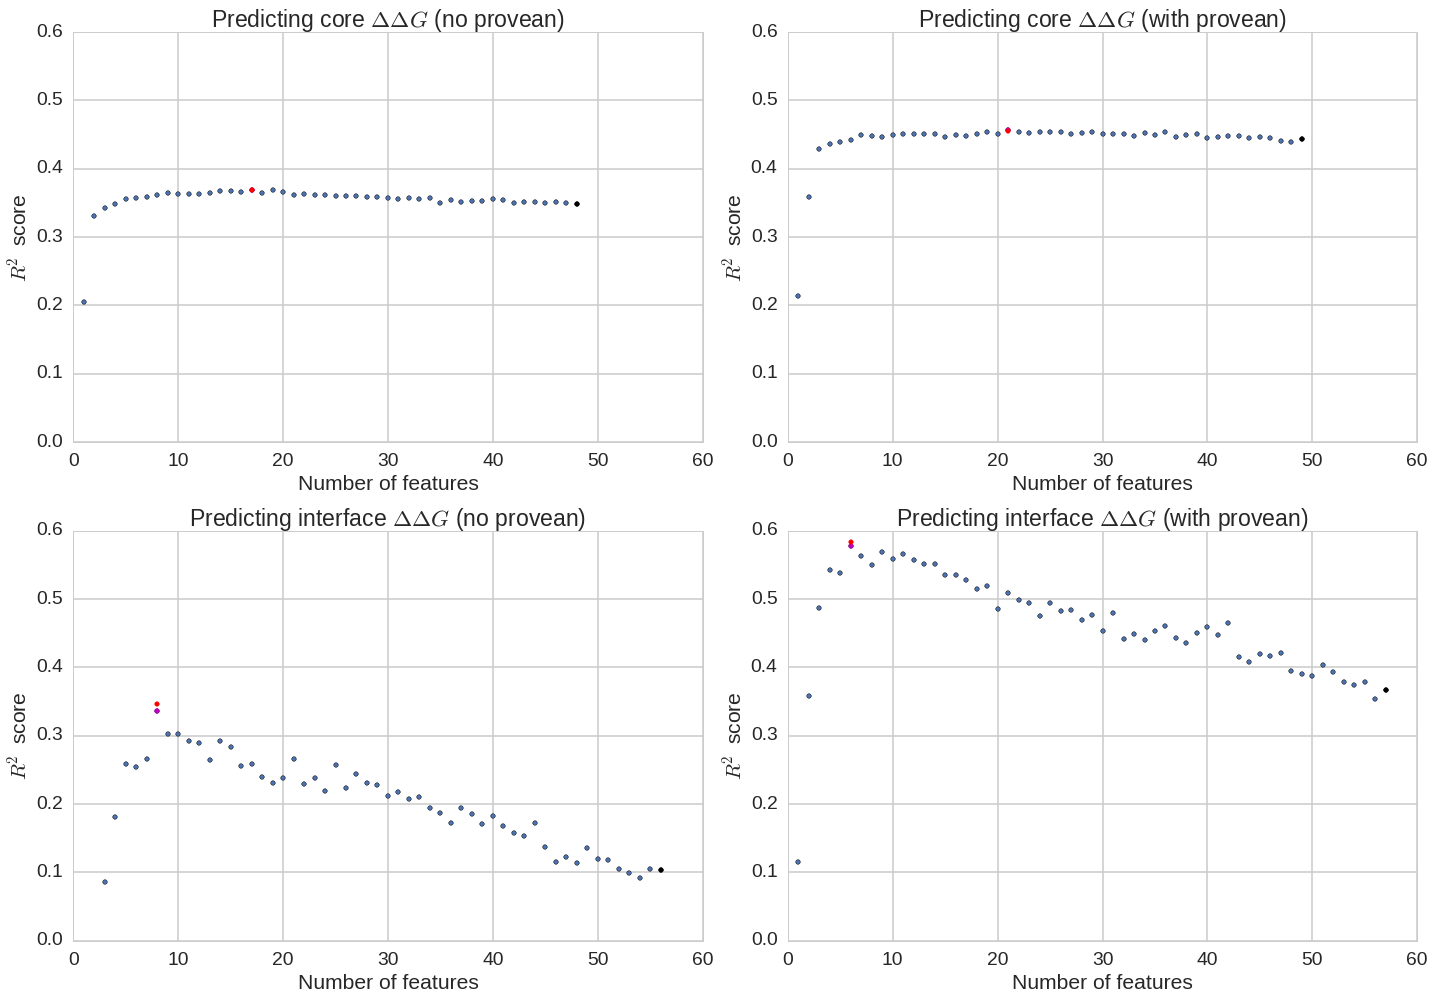
\includegraphics[scale=0.3]{image117}
	\caption{Variable elimination.}
\end{figure}

\begin{figure}[H]
	\centering
	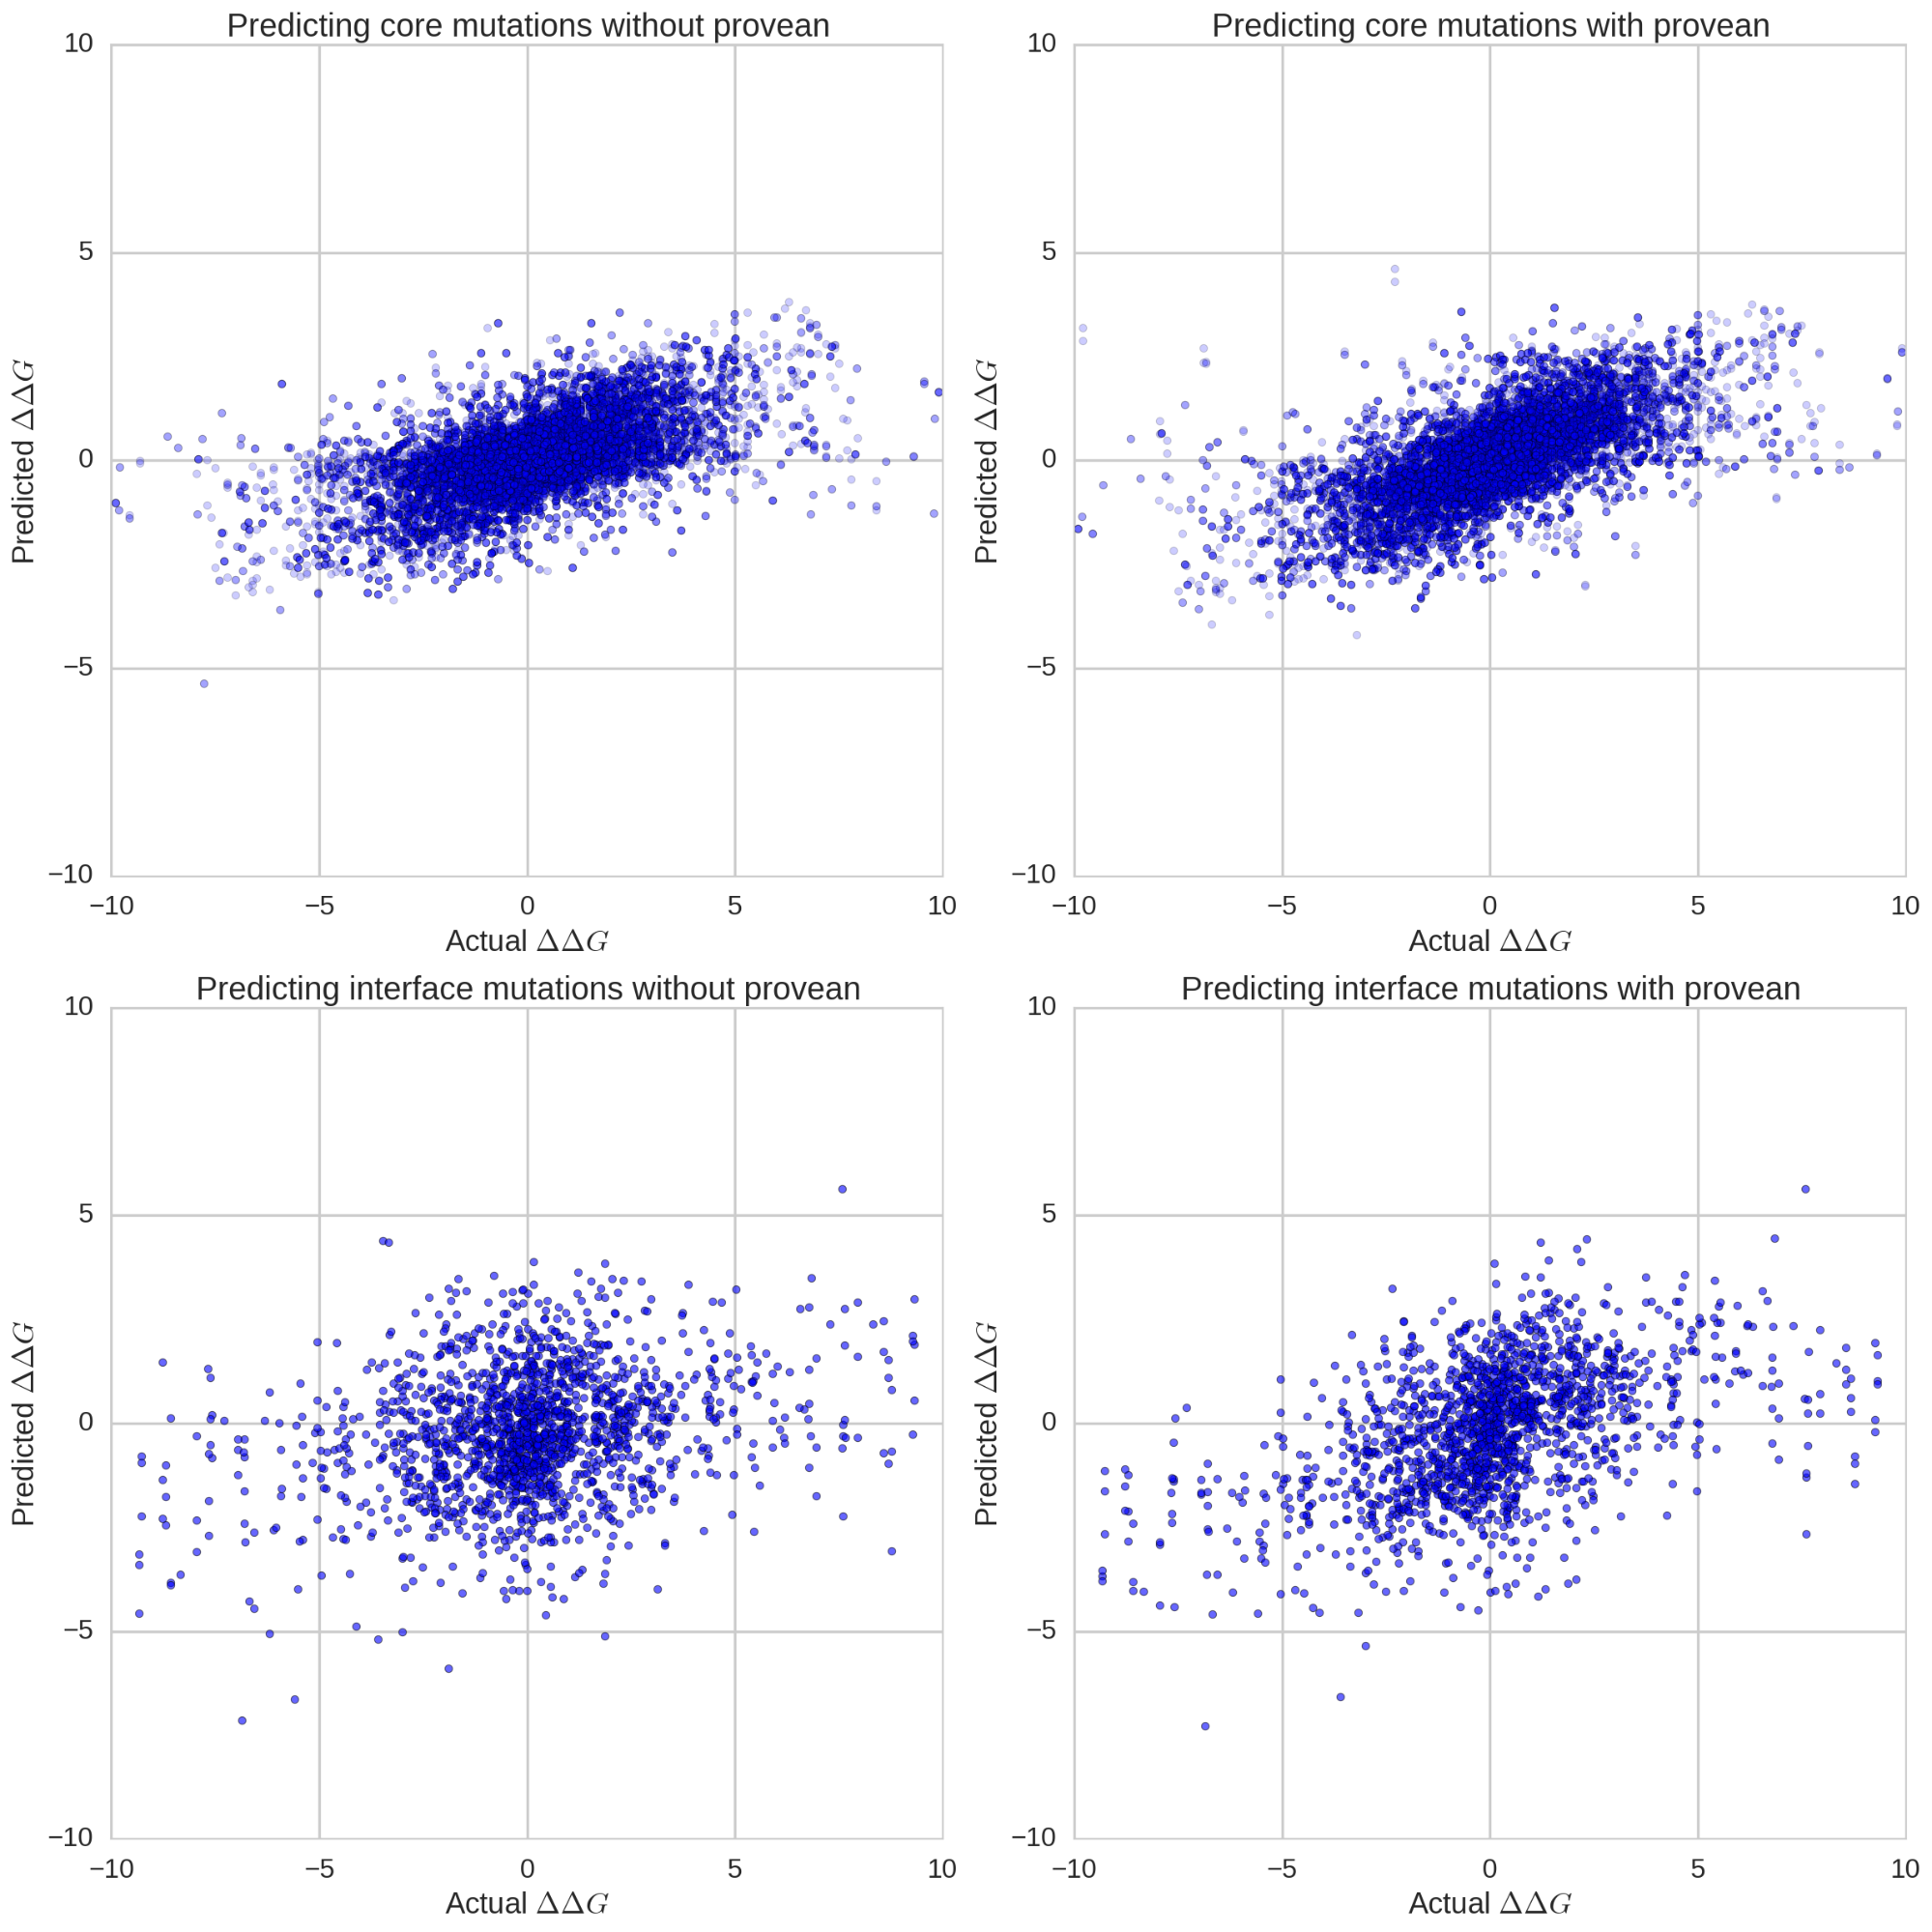
\includegraphics[scale=0.2]{image65}
	\caption{Cross-validation performance before variable elimination.}
\end{figure}

\begin{figure}[H]
	\centering
	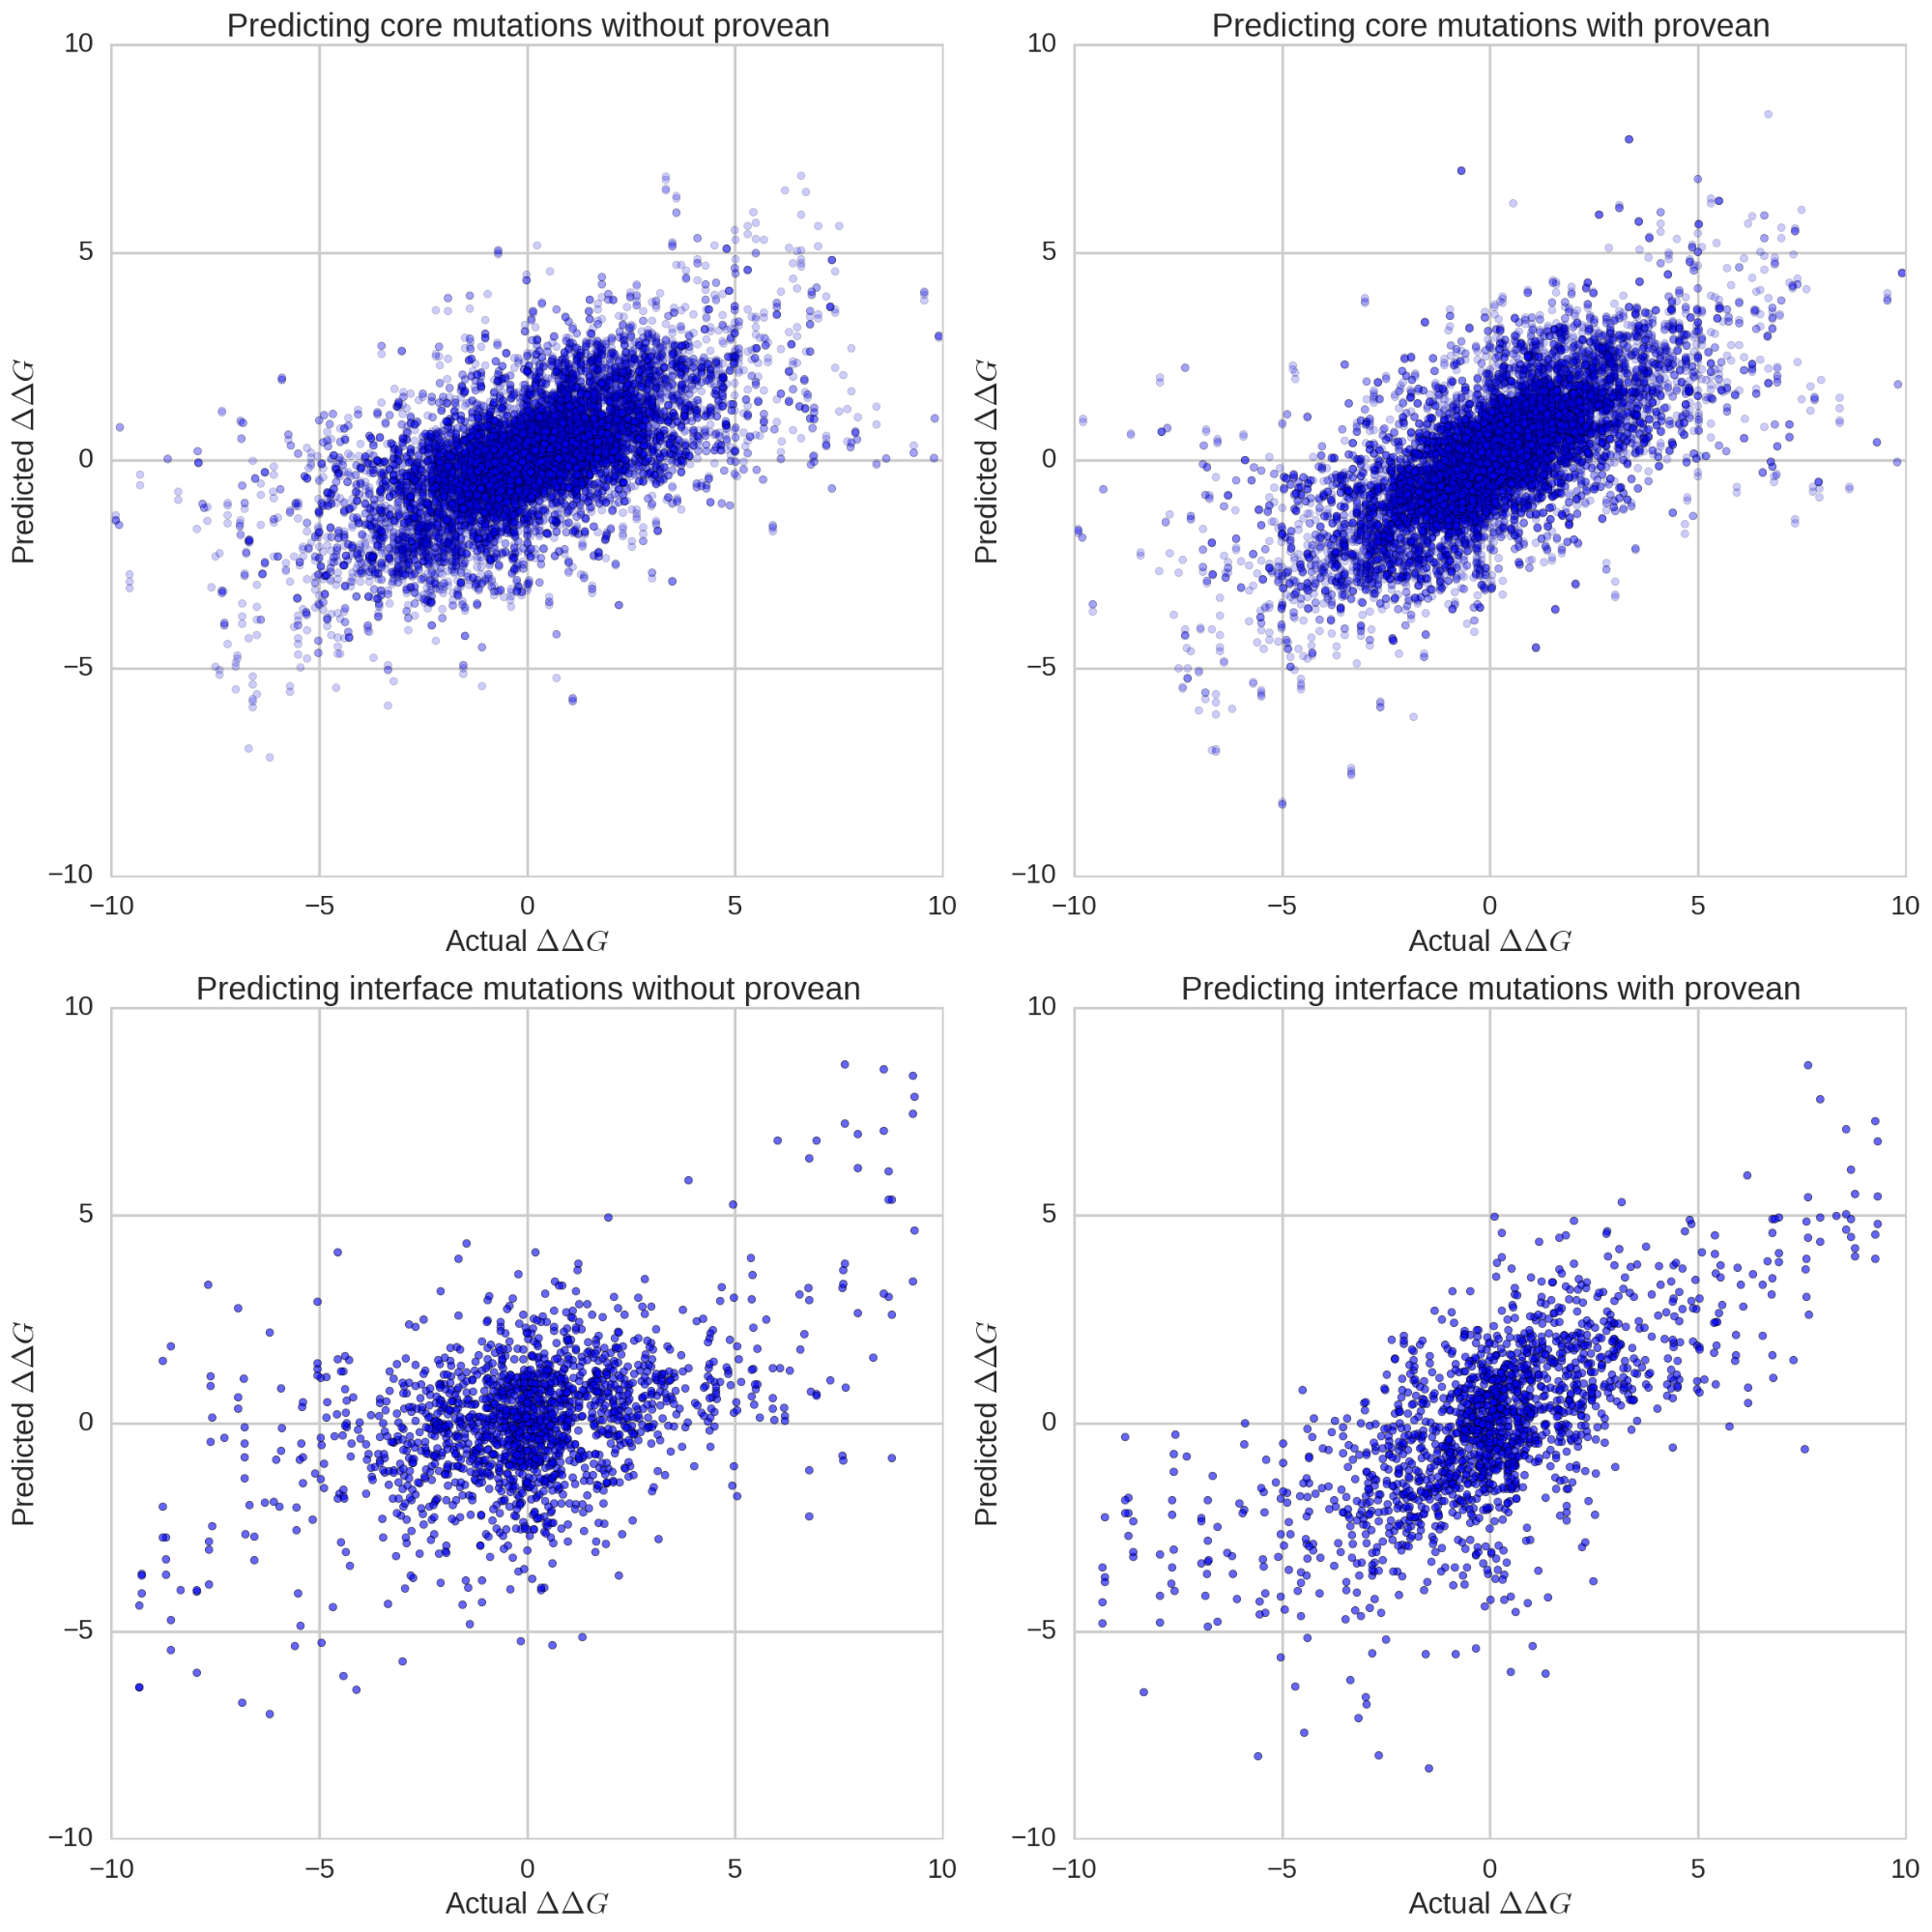
\includegraphics[scale=0.2]{image103}
	\caption{Cross-validation performance after variable elimination.}
\end{figure}

\begin{figure}[H]
	\centering
	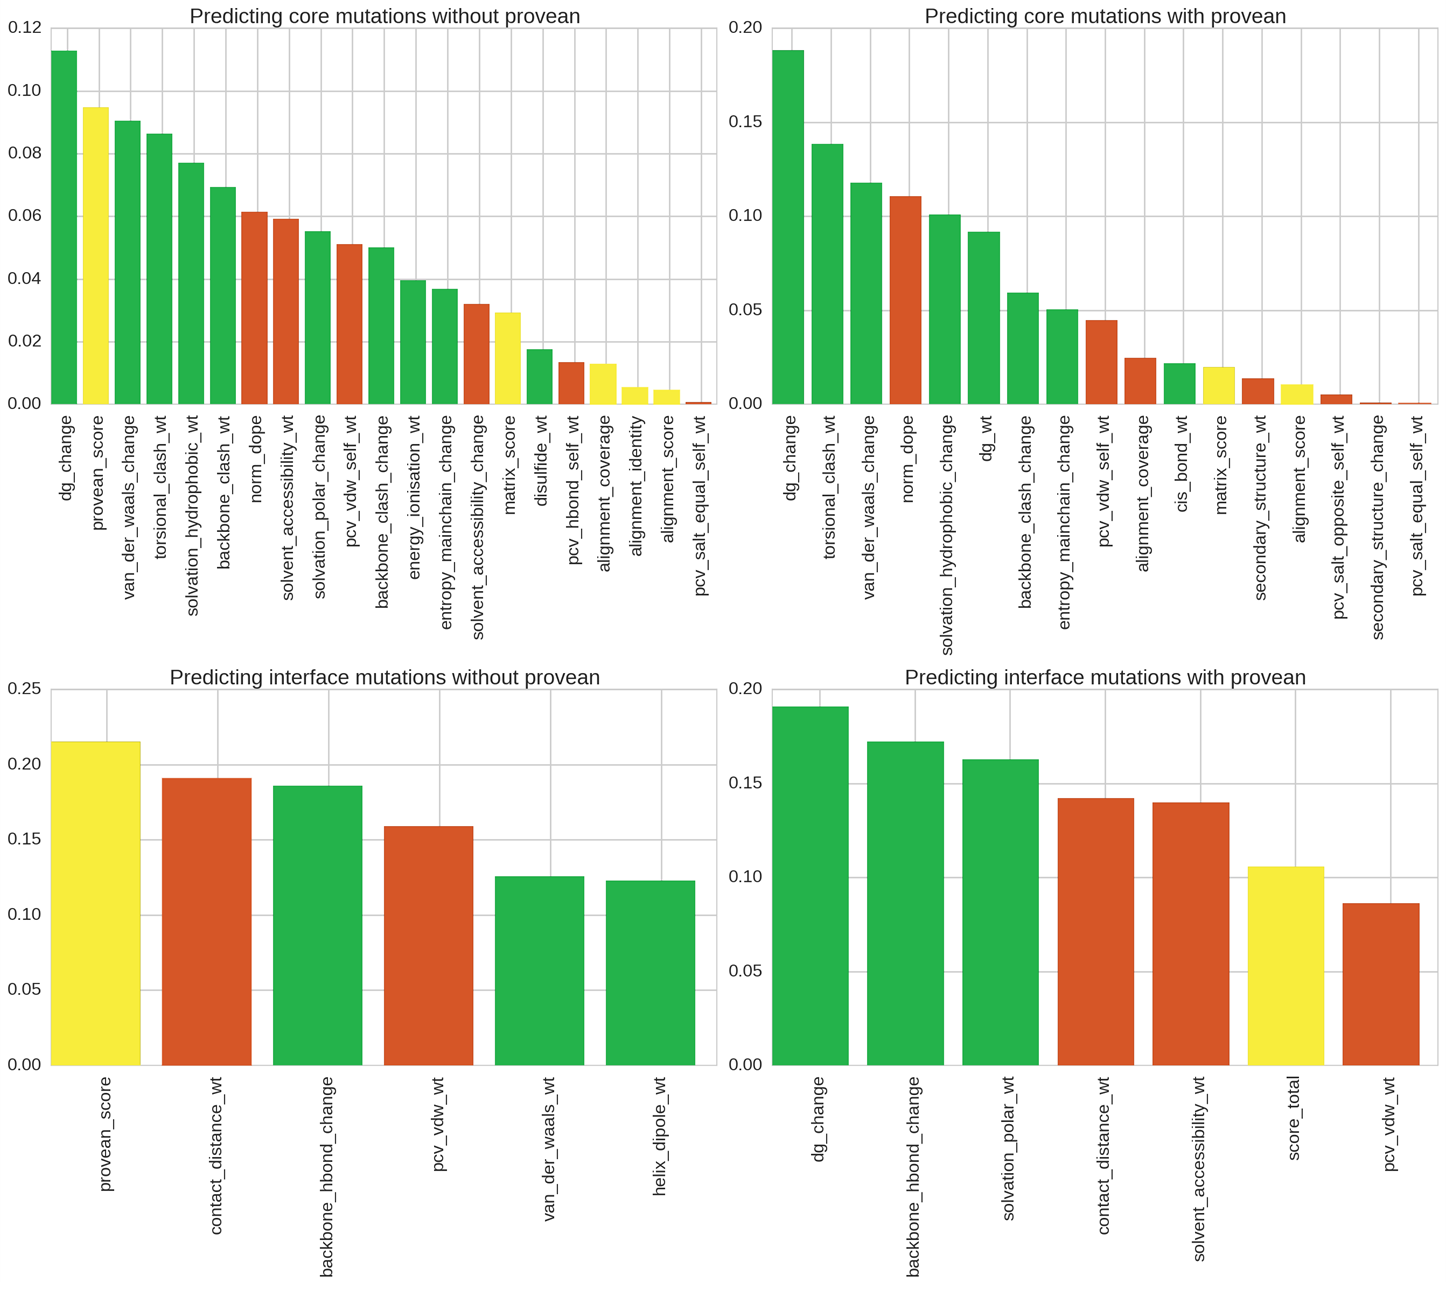
\includegraphics[scale=0.3]{image02}
	\caption{Feature importances after variable elimination.}
\end{figure}




\subsection{Validation}

Compare how well Provean, FoldX, and `ELASPIC with Provean' and `ELASPIC without Provean' distinguish between the three different datasets for both core and interface mutations.

\begin{itemize}
\item Chaperone interaction data (core mutations) \ Luciferase complementation assay (interface mutations) (use Spearman correlation coefficient).
\item Uniprot disease vs. polymorphism (use AUC / ROC / combination).
\item COSMIC driver vs. passenger.
\end{itemize}







% \subsubsection{Chaperone interaction data}
%
% \begin{figure}[H]
% 	\centering
% 	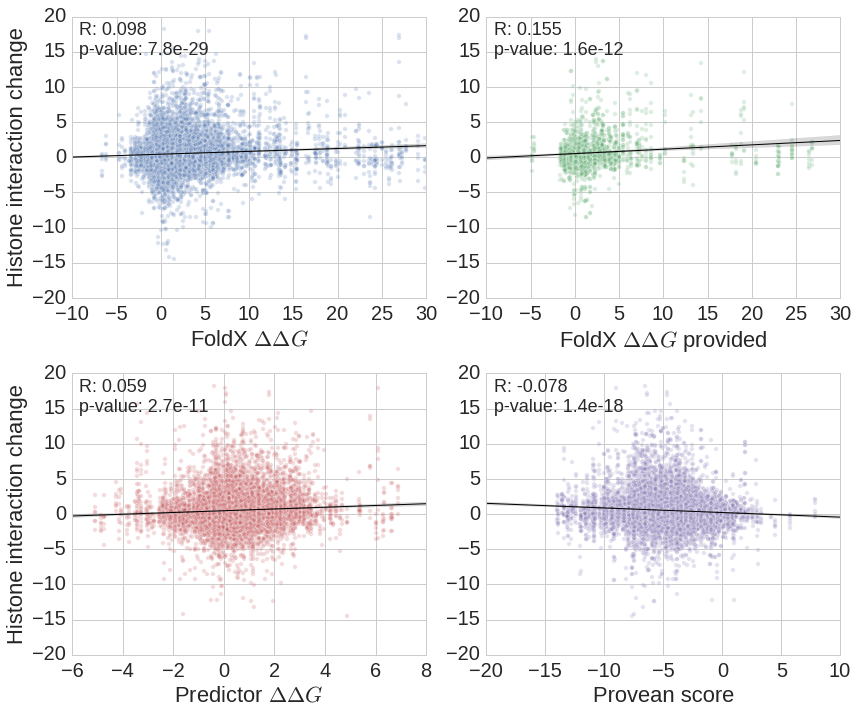
\includegraphics[scale=0.4]{image75}
% 	\caption[Core Validation]{Validation of the ELASPIC core predictor using chaperone interaction data from "Widespread Macromolecular Interaction Perturbations in Human Genetic Disorders".}
% \end{figure}
%
%
% \begin{figure}[H]
% 	\centering
% 	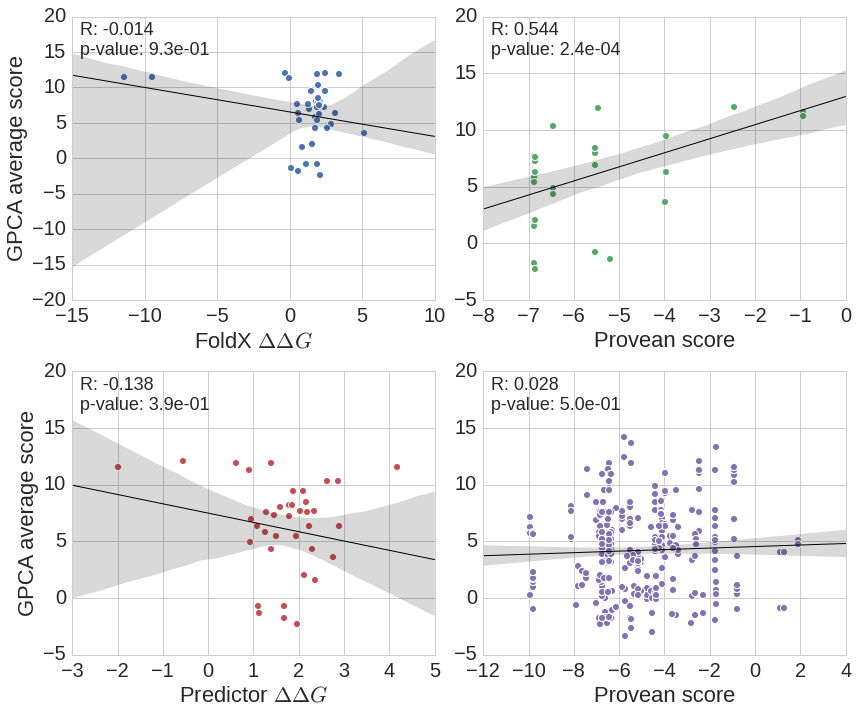
\includegraphics[scale=0.4]{image52}
% 	\caption[Interface Validation]{Validation of the ELASPIC core interface predictor using \textit{Gaussia princeps} luciferase protein complementation assay from "Widespread Macromolecular Interaction Perturbations in Human Genetic Disorders".}
% \end{figure}
%
%





\section{Structure features}

The performance of Provean is comparable to the leading mutation scoring programs, such as SITF, PolyPhen-2, Mutation Assessor, and CONDEL \cite{choi_predicting_2012}. Furthermore, Provean is distributed under a GPLv3 license, and uses \textit{supporting sets} of at most 45 sequences which can precalculated and stored. If a supporting set is available, calculating the Provean score takes several seconds per mutation.

Another widely-used mutaiton scoring tool is PolyPhen-2. It is one of the packages predicted for




\section{ELASPIC pipeline}

The ELASPIC project was started by Niklas Berliner and others in 2014 \cite{berliner_combining_2014}.

ELASPIC uses Modeller \cite{webb_comparative_2002} to construct homology models of domains and domain-domain interactions, FoldX to optimize those model and to introduce mutations \cite{schymkowitz_foldx_2005}, and the ELASPIC predictor to combine FoldX energy scores with sequence-based and other features and predict the energetic impact of a mutation on the stability of a single domain or the affinity between two domains. A flowchart describing the ELASPIC pipeline is presented in \ref{fig:elaspic_pipeline}. At each step in the pipeline, a local database is queried to see if the required information has already been calculated. If the information is available, the pipeline moves to the next step. If the information is not available, the pipeline runs the module that generates the required information, stores the generated information in the database for future access, and then moves to the next step. If the specified mutation falls outside of every domain in the protein, no predictions are returned. Otherwise, the pipeline evaluates the impact of the mutation on the stability of the domain and, if the mutation falls in a domain interface, on the affinity between two domains. In order to expedite the evaluation of mutations, we precalculated homology models and Provean supporting sets for all human proteins. Structural and sequential features, and predicted ∆∆G scores, have also been precalculated for the majority of mutations listed in the Uniprot humsavar file \cite{consortium_uniprot:_2015} and in the COSMIC \cite{forbes_cosmic:_2015} and ClinVar \cite{landrum_clinvar:_2016} databases.

Provean supporting sets, homology models and mutation ΔΔG scores are available from the ELASPIC
downloads page: http://elaspic.kimlab.org/static/download/. The source code of the python package implementing the ELASPIC pipeline is available from https://github.com/kimlaborg/elaspic, and the documentation for the ELASPIC pipeline can be accessed online at http://elaspic.readthedocs.org/.


\section{ELASPIC web service}

\begin{table}[H]
	\centering
	\caption{ELASPIC web service API.}
	\label{my-label}
	\begin{tabular}{lll}
	\textbf{Method} & \textbf{HTTP request} & \textbf{Description} \\
	submitjob & POST /submitjob & Submit a job to be run on a SGE cluser. \\
	jobstatus & GET /submitjob & View the results of a job.
	\end{tabular}
\end{table}

\chapter{Results}

% !TEX root = msc_thesis.tex

\chapter{Discussion}

\section{Limitations}

Cystic fibrosis

  - Existing approaches remain limited in their ability to predict disease-causing variants. In a study of 1571 mutations of the CFTR gene causing cystic fibrosis, (SIFT, PolyPhen, PANTHER) \cite{dorfman_common_2010}

Long QT syndrome

  - Assessment of the predictive accuracy of five in silico prediction tools, alone or in combination, and two metaservers to classify long QT syndrome gene mutations.

  - http://www.ncbi.nlm.nih.gov/pubmed/25967940



\section{Future Directions}

% Improve domain definitions and alignments

eSCOP

Gene3D

- Use sequence profiles (e.g. Pfam or Gene3D) to guide the alignment.


\subsection{Better features}


% Better features

- Use covariation between amino acids in addition tho the conservation score to predict the impact of mutations, as described by Kowarsch et. al. \cite{kowarsch_correlated_2010}. \\


% Replace FoldX with MODELLER

- Use multiple templates when building the homology models. \\
- Create multiple models and choose the one with the highest DOPE score. \\
- Refine the model using molecular dynamics. \\

Long-term MD is not useful for optimizing structures in most cases \cite{raval_refinement_2012}.



\subsection{Mutation affecting multiple amino acids}

ELASPIC can easily be extended to calculate the $\Delta \Delta G$ for mutations invovling multiple amino acids. The tricky part is that the number of features changes with the number of amino acids that are mutated. We could address this by treating a mutation affecting multiple amino acids as a set of single amino acid mutations. For example, we could use the following recursive strategy:

\begin{enumerate}
    \item Introdue each of the single amino acid mutations, one at a time.
    \item Select the single amino acid mutation with the most stabilising effect.
    \item Repeat for the remaining mutations, using the structure containing the mutation selected in Step 2.
\end{enumerate}

About one third on mutations in the Protherm and Skempi databases affect multiple amino acids. We could include those mutations in the training set by dividing them into single amino acid mutations and assigning to them a $\Delta \Delta G$ proportional to their contribution to the overall mutation score, as determined by the multiple amino acid substitution version of ELASPIC. This would require ``bootstrapping'' the ELASPIC predictor using single amin acid mutations, using the ``bootstrapped'' predictor to approximate the contribution of single amino acid mutaitons to the $\Delta \Delta G$ affecting mulitple amino acids, adding those mutations to the training set, and repeating.

It is likely that the performance of the ELASPIC predictor would be lower for mutations affecting multiple amino acids than for mutations affecting a single amino acids, as the former is more likely to induce changes in the conformation of the protein that are not modelled by ELASPIC. The performance of ELASPIC could potentially be improved by including a backbone relaxation step between each mutation, using molecular dynamics \cite{abraham_gromacs:_2015}, backrub \cite{smith_predicting_2011}, or other algorithms \cite{sun_protein_2016}.

If the ELASPIC preictor can achieve reasonable results for mutations affecting multiple amino acids, it could be used ``in reverse'' to design protein domains with increased stability and protein interfaces with increased affinity.


% Multiple mutations + insertions / deletions

- Predict homo-oligomers, since this is the predominant form of oligomerization in proteins. \\
- Multiple amino acid substitutions + insertions / deletions. \\
- Alternative splicing / aberrant splicing. \\


% Protein-protein interactions

Predict PPIs: PRISM: Protein interaction by structure matching.



% Protein-ligand interactions

- drugging protein-protein interfaces \cite{wells_reaching_2007}

Platinum: Protein-ligand affinity change upon mutation database.

  - http://bleoberis.bioc.cam.ac.uk/platinum/


BioLiP is a semi-manually curated database for high-quality, biologically relevant ligand-protein binding interactions.

  - http://zhanglab.ccmb.med.umich.edu/BioLiP/

  - The structure data are collected primarily from the Protein Data Bank, with biological insights mined from literature and other specific databases.



% Protein-DNA/RNA interactions

ProNIT



% Protein-peptide interactions

ELM


%% This adds a line for the Bibliography in the Table of Contents.
\addcontentsline{toc}{chapter}{Bibliography}
%% *** Set the bibliography style. ***
%% (change according to your preference/requirements)
%\bibliographystyle{plain}
%% *** Set the bibliography file. ***
%% ("thesis.bib" by default; change as needed)
% \bibliography{msc_thesis}

% AS References
% \printbibheading
\printbibliography[title={Bibliography}]


%% *** NOTE ***
%% If you don't use bibliography files, comment out the previous line
%% and use \begin{thebibliography}...\end{thebibliography}.  (In that
%% case, you should probably put the bibliography in a separate file and
%% `\include' or `\input' it here).

\end{document}
